\documentclass[12pt]{article}
\usepackage[utf8]{inputenc}
\usepackage{graphicx}
\usepackage{geometry}
\usepackage{float}
\usepackage{listings}
\usepackage{xcolor}
\geometry{a4paper, margin=1in}

\lstset{
	basicstyle=\ttfamily\small,
	backgroundcolor=\color{lightgray},
	frame=single,
	breaklines=true,
	tabsize=2,
	numbers=left,
	numberstyle=\tiny,
	numbersep=5pt,
	keywordstyle=\color{blue}\bfseries,
	commentstyle=\color{green},
	stringstyle=\color{red},
	showstringspaces=false,
}

\begin{document}
	% Title Page
	\begin{titlepage}
		\centering
		\vspace*{5cm}
		
\includegraphics[width=0.5\textwidth]{profile.png}\\[1cm]
		\Huge
		\textbf{Image Processing, Word Cloud, and Network Analysis}\\[1cm]
		\Large
		\textbf{Mahdiyeh Ebrahimy}\\
		Student ID: 4011290481\\[2cm]
		\vfill
		\large
		January 2025
	\end{titlepage}
	
	
	\tableofcontents
	\newpage
	
	% Image Processing Section
	\section{Image Processing}
	In this section, we demonstrate how an image was processed using R, including resizing, splitting, and annotating the image.
	\subsection*{Code}
	\begin{lstlisting}[language=R]
		options(warn = -1)
		library(ggplot2)
		library(grid)
		library(magick)
		image_path <- "ShowPic.png"
		
		original_image <- image_read(image_path)
		
		# Resize and process image
		resized_image <- image_scale(original_image, "400x400")
		image_width <- as.numeric(image_info(resized_image)$width)
		image_height <- as.numeric(image_info(resized_image)$height)
		left_half <- image_crop(resized_image, paste0(image_width / 2, "x", image_height, "+0+0"))
		right_half <- image_crop(resized_image, paste0(image_width / 2, "x", image_height, "+", image_width / 2, "+0"))
		right_half <- image_convert(right_half, colorspace = "gray")
		combined_image <- image_append(c(left_half, right_half), stack = FALSE)
		final_image <- image_annotate(combined_image, "The next president of Taiwan", size = 20, gravity = "north", color = "orange", boxcolor = "black")
		#I just dont have any islamic pic
		knitr::include_graphics("processed_image.png")
		
		# پردازش تصاویر RGB و ایجاد انیمیشن
		resized_image <- image_scale(original_image, "600x400")
		r_image <- image_modulate(resized_image, brightness = 100, saturation = 100, hue = 0)
		g_image <- image_modulate(resized_image, brightness = 100, saturation = 100, hue = 120)
		b_image <- image_modulate(resized_image, brightness = 100, saturation = 100, hue = 240)
		
		# چرخش و تغییر اندازه برای ایجاد انیمیشن
		r_image_rotated <- image_scale(image_rotate(r_image, 90), "150x150")
		g_image_rotated <- image_scale(image_rotate(g_image, 180), "300x325")
		b_image_rotated <- image_scale(image_rotate(b_image, 0), "300x325")
		
		# ایجاد انیمیشن GIF
		rgb_animation <- image_animate(c(g_image_rotated, b_image_rotated, r_image_rotated), fps = 1)
		image_write(rgb_animation, path = "rgb_animation.gif", format = "gif")
		library(magick)
		animation <- image_read("rgb_animation.gif")
		image_write(animation, path = "frame_%02d.png", format = "png")
		
		# نمایش انیمیشن در HTML
		knitr::include_graphics("rgb_animation.gif")
		
	\end{lstlisting}

	\begin{figure}[H]
		\centering
		
\includegraphics[width=0.4\textwidth]{ShowPic.png}
		\caption{Original Image}
	\end{figure}
	 		\newpage
	
	
	
	
	
	
	The processed image with annotation is shown below:
	\begin{figure}[H]
		\centering
		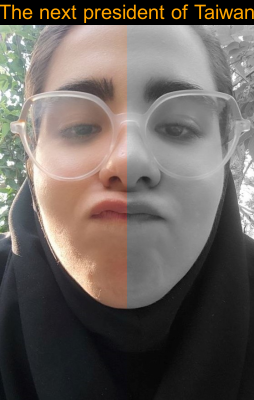
\includegraphics[width=0.4\textwidth]{processed_image.png}
		\caption{Processed Image with Annotation}
	\end{figure}
	
	\newpage
	% Word Cloud Section
	\section{Word Cloud}
	In this section, we generated a word cloud from the titles of news articles using the provided dataset. The most frequently occurring words are highlighted.
	\subsection*{Code}
	\begin{lstlisting}[language=R]
	library("NLP")
	library("tm")
	library("SnowballC")
	library("RColorBrewer")
	library("wordcloud")
	
	data <- read.csv("FakeNewsNet.csv", stringsAsFactors = FALSE)
	text <- na.omit(data$title)
	text <- text[1:1000]
	docs <- Corpus(VectorSource(text))
	toSpace <- content_transformer(function(x, pattern) gsub(pattern, " ", x))
	docs <- tm_map(docs, toSpace, "/")
	docs <- tm_map(docs, toSpace, "@")
	#docs <- tm_map(docs, "\\|", toSpace)
	docs <- tm_map(docs, content_transformer(tolower))
	docs <- tm_map(docs, removeNumbers)
	docs <- tm_map(docs, removeWords, stopwords("english"))
	docs <- tm_map(docs, removePunctuation)
	docs <- tm_map(docs, stripWhitespace)
	dtm <- TermDocumentMatrix(docs, control = list(wordLengths = c(3, Inf)))
	m <- as.matrix(dtm)
	v <- sort(rowSums(m), decreasing = TRUE)
	d <- data.frame(word = names(v), freq = v)
	png("wordcloud.png", width = 800, height = 600)
	knitr::include_graphics("wordcloud.png")
	wordcloud(words = d$word, freq = d$freq, min.freq = 1, max.words = 75, random.order = FALSE, rot.per = 0, scale = c(2.4, 0.35), colors = brewer.pal(8, "Dark2"))
	dev.off()
	\end{lstlisting}
	
	\begin{figure}[H]
		\centering
		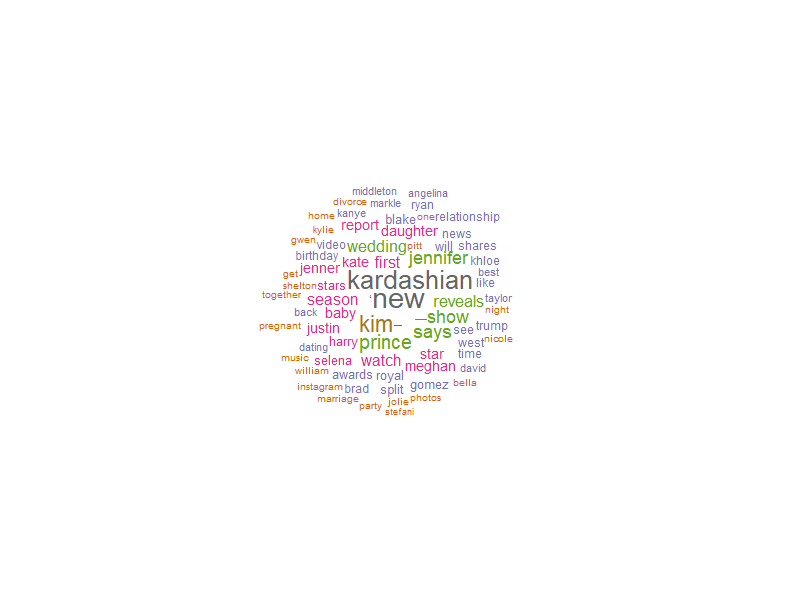
\includegraphics[width=\textwidth, keepaspectratio]{wordcloud.png}
		\caption{Generated Word Cloud}
	\end{figure}
	
	
	\newpage
	
	% Network Analysis Section
	\section{Network Analysis}
	This section analyzes a dataset of relationships, creating a network graph to visualize connections between nodes (teams or entities).
	\subsection*{Code}
	\begin{lstlisting}[language=R]
	library(igraph)
	file_path <- "results.csv"
	data <- read.csv(file_path)
	data <- subset(data, tournament == "AFC Asian Cup")
	data <- data.frame(winner = ifelse(data$home_score > data$away_score, data$home_team, data$away_team), loser = ifelse(data$home_score > data$away_score, data$away_team, data$home_team), date = as.Date(data$date))
	library(dplyr)
	y <- data %>% group_by(winner, loser) %>% summarise(weight = n(), .groups = 'drop')
	y <- y %>% arrange(winner, loser) %>% filter(!duplicated(paste(pmin(winner, loser), pmax(winner, loser))))
	net <- graph.data.frame(y, directed = TRUE)
	V(net)$label <- V(net)$name
	V(net)$degree <- degree(net, mode = "all")
	net <- delete.vertices(net, V(net)[degree(net, mode = "out") < 5])
	png("network_graph.png", width = 800, height = 600)
	knitr::include_graphics("network_graph.png")
	plot(net, layout = layout_with_fr, vertex.color = rainbow(length(V(net))), vertex.size = log(V(net)$degree + 1) * 6, edge.arrow.size = 0.3, vertex.label.cex = 0.8, vertex.label.color = "black", main = "AFC Asian Cup Network Graph")
	dev.off()
	knitr::include_graphics("network_graph.png")
	\end{lstlisting}
	
	\begin{figure}[H]
		\centering
		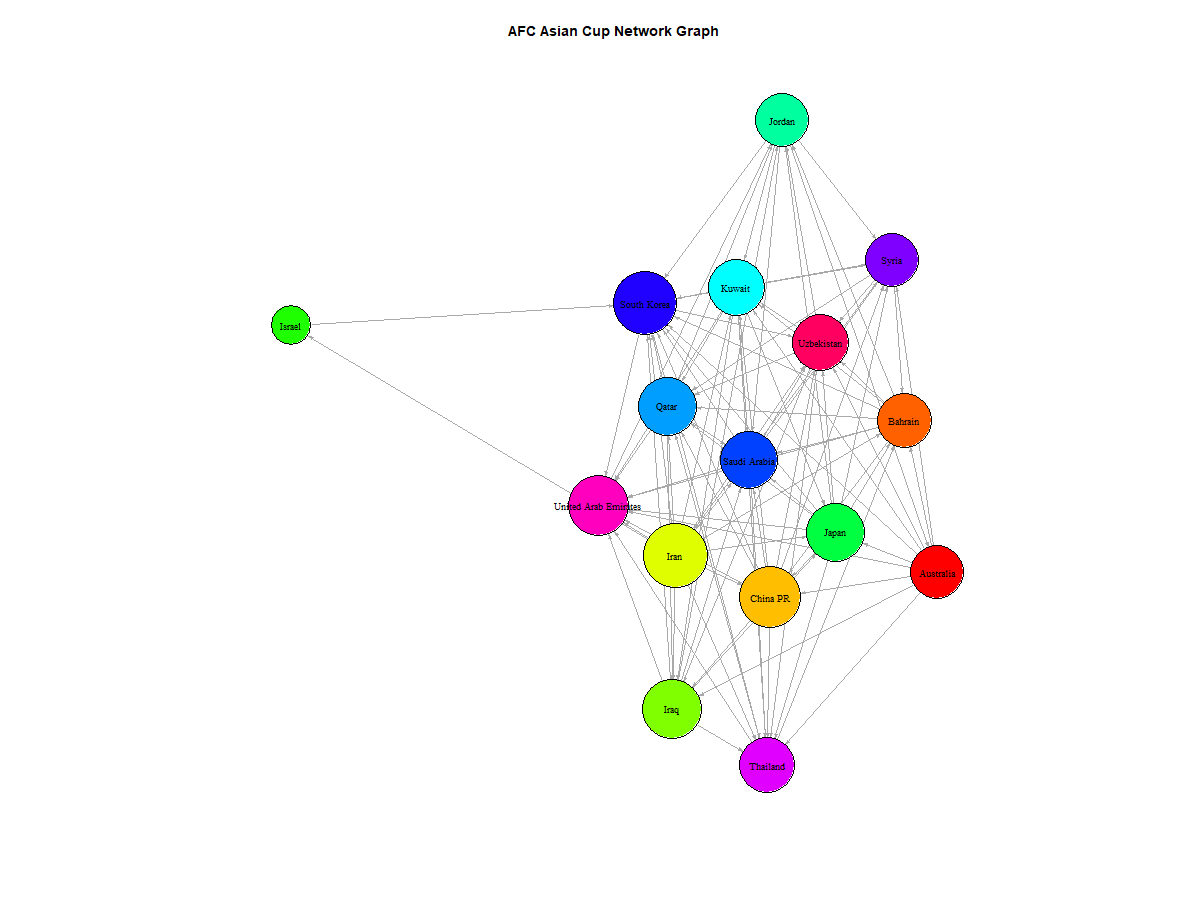
\includegraphics[width=1\textwidth]{network_graph.png}
		\caption{Network Analysis Graph}
	\end{figure}
	
\end{document}
